\section{Native closure, wave and temporal fixtures}
\label{manual:m1-native-fixtures}
The executable motif and fold fixtures use a declared preassembled-prefix
realization: component closures complete before the target trace starts.
This is a sufficient causal realization of the Main's more general
commit-before-consumption rule. Each outer trace binds its inner identity,
certificate set and scope map before certification. A further distinct outer
return supplies the outer beat; exposure preserves the bound inner wave.
Duon fixtures separately execute the twelve support signatures, carried current,
distinct recurrent returns and the Duad's seated state of the same identity.
The finite harmonic readout declares a cyclic index group and committed window;
every recorded state contains only the certificate, cadence and phase prefix
available at that return. Its projection is a declared model record.
\paragraph{Record class and execution.}
These are native exact witnesses or explicitly declared models. The shared
runner is \texttt{manual/scripts/aod\_native\_closure\_wave.py}; its five CSV
inputs preserve trace, scope, lineage, expected exact result and hostile case.
The command \texttt{python3 manual/scripts/aod\_native\_closure\_wave.py --check-data}
executes the rows. An expected rejection is a successful hostile check only
when the actual law rejects the supplied input. Actual results are recorded
separately from these immutable inputs.

\begin{longtable}{p{0.23\linewidth}p{0.33\linewidth}p{0.34\linewidth}}
\toprule Construction & Exact witness & Hostile control\\\midrule
Null/anchor & Five distinct types; first \(00_8\) & Prior coordinate choice or type collapse\\
Atomic support & H1 legs, composite H2 and closed H0 endpoints & Direct H2 called atomic\\
Hinge/phase & \(\varepsilon0_H(0_D)^m(-\varepsilon)\), \(m=0,2\), one phase & Bypass, same-sign end, replay recount\\
Reflected legs & \(1+1=2\), \(1+3=4\); unit embedding \(1_C\mapsto2h\) & Unequal-leg factorization; missing witness\\
Recurrence & Three bound closures give two beats, separations \((10,10)\) & One closure or repeated certificate\\
Kernel & Weights \((1,1)\) or \((1,3)\) on admitted support & Bypass mass; empty normalization\\
Motifs & Dion, two-Monon Dimonon, 12 Duon variants, Duad state & Collapsed names or changed certificate bytes\\
Fold/exposure & One outer phase, retained inner wave & Contact called closure; lower beats reused\\
Temporal pair & Ratio, bias, unwrapped lag, directional RCD & Aliases, one contact, zero denominator\\
State/update & Equal temporal view, different pressure; later response & Future input or projection/state collapse\\
Flux/Stokes & AFC \(0\) or \(1/2\); AOD \(7\), boundary \(3\) & Pressure in normalized memory; wrong reverse sign\\
FRG & Independent \(5\), cross \(3\), recurrent \(8\) & Model before admission; same-step response\\
Harmonics & \((1,0,-1,0)\) reconstructs exactly & Unbound word gains admission\\
Conservation & Active one-phase equation binding & Mapping that source to an unrelated Fourier equation\\
Report & \(Nn=3(2/3)=2\), \(4(2/3)=8/3\) & Missing calibration; \(3n\) used for \(N=4\)\\
\bottomrule
\end{longtable}

\paragraph{Directional count realization.}
Both wave identities and repeated contact-prefix digests are bound before
comparison. With support \(RD=3\) and two reflection counts, the declared
additive interface gives \(\rho^D_{a|b}=3+1+1=5\) and
\(\rho^D_{b|a}=3+2+2=7\). The ratio reverses reciprocally, signed offsets
reverse, and the directional duration is recomputed. A same-domain window of
two clips only participation to two; it changes neither RD nor RCD.
The native count comparator has \(\Lambda=N_a-N_b+b_a-b_b\), with drift
formed against the preceding committed comparison. A whole-closure slip
changes this unwrapped value even when a separately wrapped display repeats.

\paragraph{Interface composition.}
A recurrent \(8\to9\to8\) realization initializes at vertex 8 and composes
with the committed-return readout. Primitive Duon components and targets share
their resolution; cross-scale composition uses the explicit folding map.
The comparison takes precisely two rational offsets; contact commitments,
window endpoints and update cuts are integers. Contacts use closed window
support \([u,v]\), while return counts use \((u,v]\). A lineage retains its ancestor identity
under a fixed coordinate relabelling; a substituted ancestor is rejected.
Every outer certificate carries the admitted inner waves and their bound
scope map. The controls reject missing fold provenance, unrelated-scale
pivots, malformed windows and fractional cuts, preserving rational currents.
These controls run with \texttt{python3 -m pytest -q}
\texttt{tests/test\_native\_closure\_wave.py}.

\paragraph{Calibrated report boundary.}
The emitter/mirror record uses \(N=\Delta\mathrm{bip}_{\mathrm{return}}\) and
\(x^{\mathrm{mir}}=Nn\). The displayed \(x=3n\) is restricted to \(N=3\).
A metrology record declares measurand, protocol, reference realization,
coupling/probe, detector, calibration, unit, resolution, uncertainty,
repeatability and traceability. The rational multiplier in this demonstration
is a declared report calibration, not an empirical calibration or native time unit.

\aodprovenance{main:eq:first-anchor; main:eq:atomic-h1;
main:eq:closure-certificate; main:eq:closure-phase; main:eq:return-identity;
main:eq:cumulative-closure-counts; main:eq:closure-phase-window;
main:eq:wave-identity; main:eq:reflected-leg-bound; main:eq:motif-admission;
main:eq:field-organization; main:eq:fold-outer-closure;
main:eq:relational-time; main:eq:rcd-coupling; main:eq:flux-types;
main:eq:causal-update; main:eq:fourier-transform.}
\subsection{Cycle-shedding demonstration}
\label{app:cycle-shedding-demonstration}

\subsection{Scope}
\label{app:cycle-shedding-demo-scope}
This demonstration run illustrates boundary accounting after the ontology has been declared. It uses one temporal cycle group on one retained field and records lead--lag span, temporal SADAR burden, sheddic excess, outward remainder, local reclosure, and sheddic path triggers.

\subsection{Setup}
\label{app:cycle-shedding-demo-setup}
For tick \(t\), let \(L_t\) be the lead component, \(G_t\) the lag component, \(S_t\) the disturbance span, \(P_t\) the burden, \(C_t\) local closure compatibility, \(X_t\) sheddic excess, \(O_t\) outward remainder, and \(R_t\) local reclosure.

\subsection{Statement(s)}
\label{app:cycle-shedding-demo-statements}
\[
S_t=|L_t-G_t|,
\qquad
\widetilde P_t=\eta_{\mathrm{ret}} P_{t-1}+\gamma_{\mathrm{span}} S_t,
\]
\[
X_t=\max(0,\widetilde P_t-C_t),
\qquad
P_t=\widetilde P_t-X_t,
\]
\[
O_t=(1-\lambda_{\mathrm{reclose}})X_t,
\qquad
R_t=\lambda_{\mathrm{reclose}}X_t.
\]
Here \(O_t\) is the non-reclosed outward remainder; route placement may later split it into exoshedding, redirected support routing, and open loss.

\subsection{Demonstration}
\label{app:cycle-shedding-demo-demonstration}
The displayed run uses \(90\) ticks, retention coefficient \(\eta_{\mathrm{ret}}=41/50\), span gain \(\gamma_{\mathrm{span}}=11/20\), and reclosure fraction \(\lambda_{\mathrm{reclose}}=19/50\). The lead and lag components are declared deterministic test streams with two local disturbance pulses.

\begin{figure}[H]
\centering
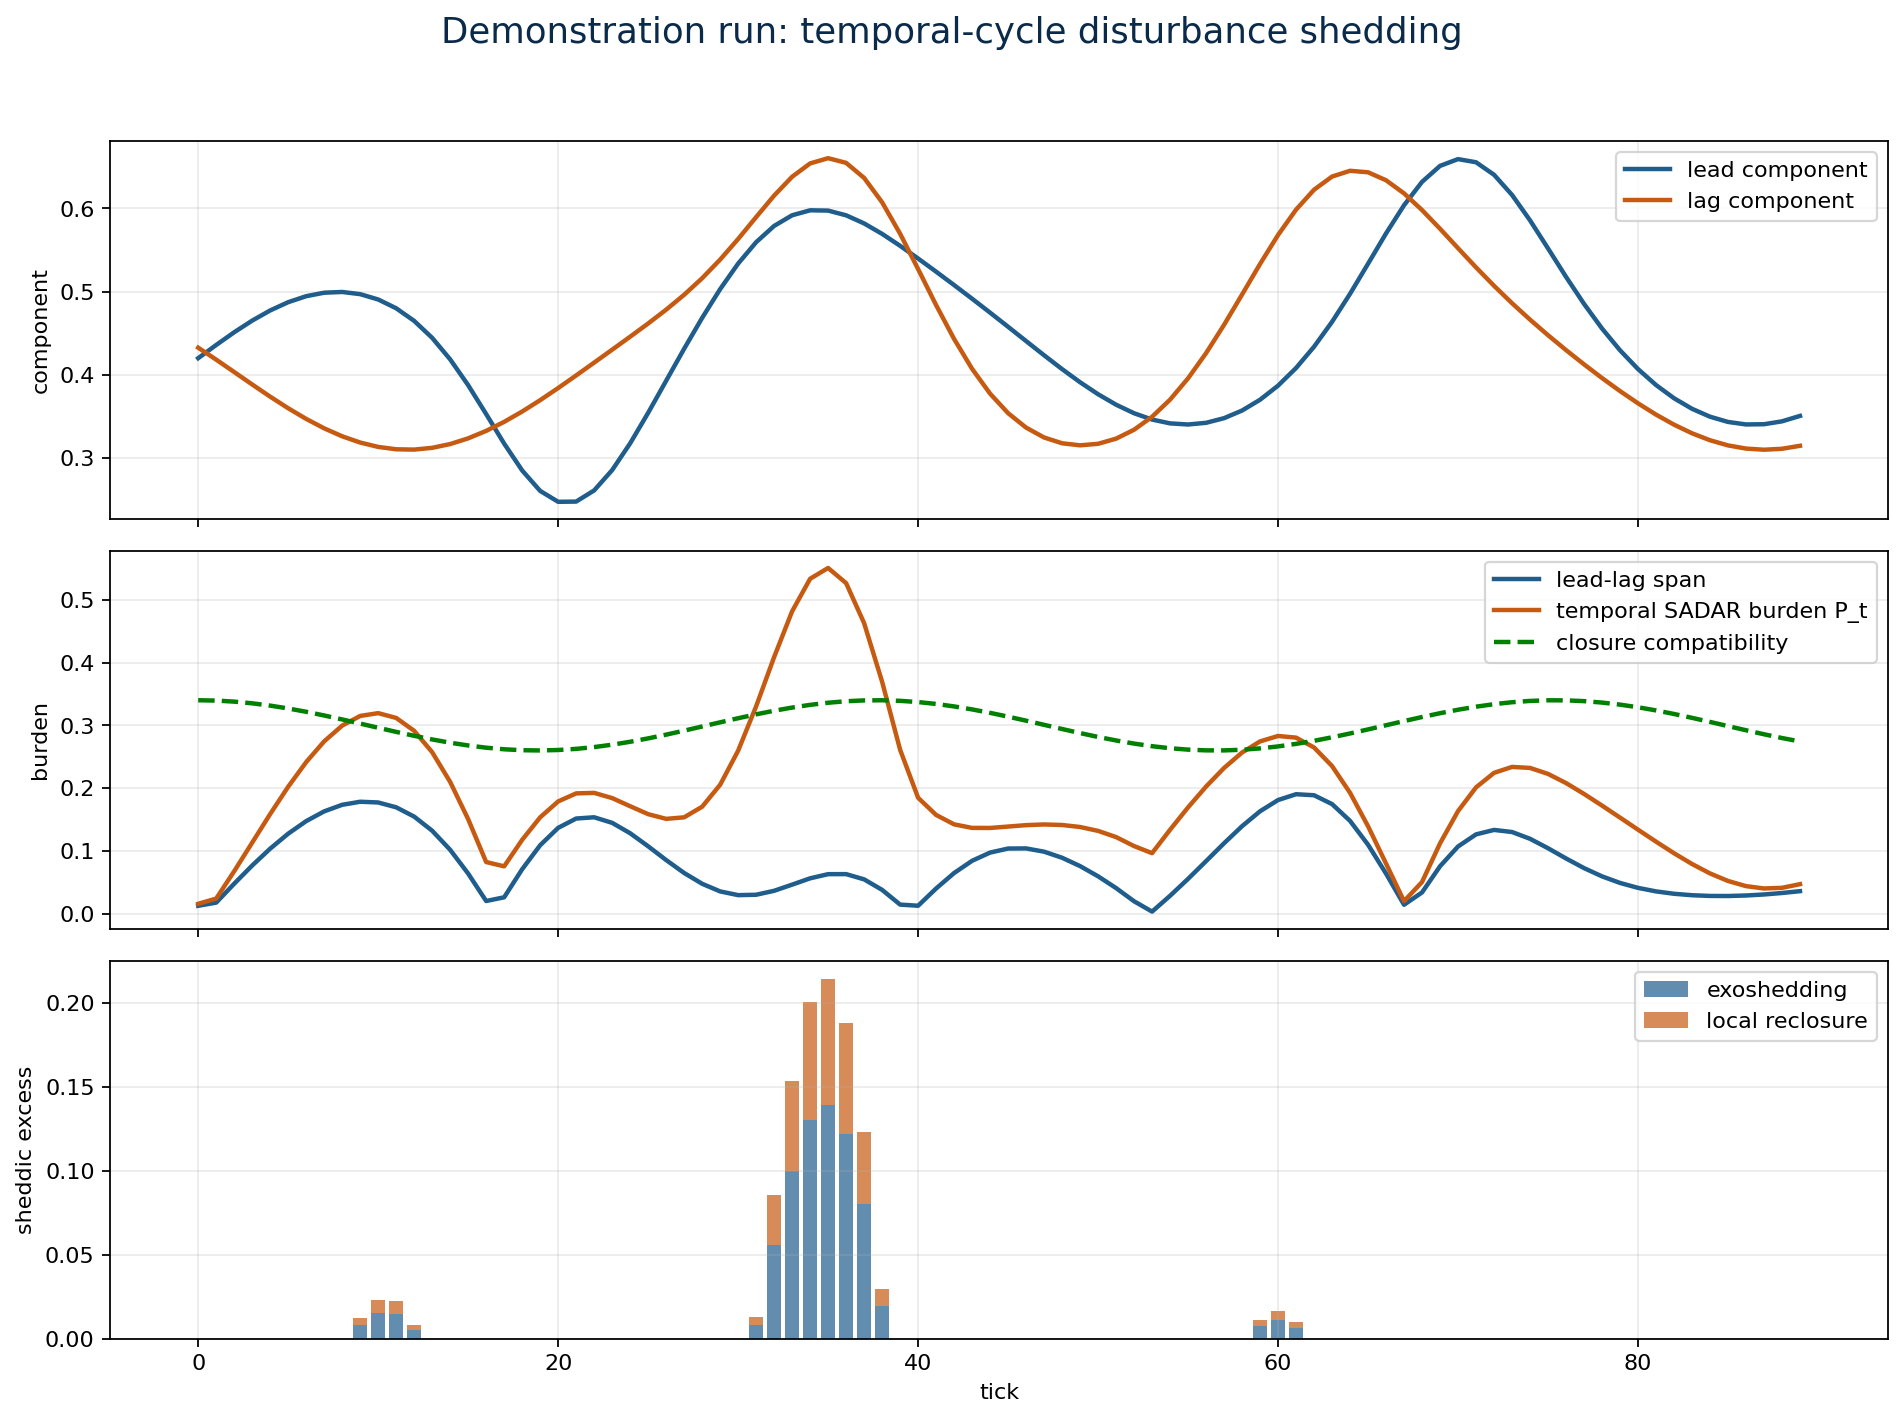
\includegraphics[width=0.98\linewidth]{../figures_jpg/cycle_disturbance_shedding_simulation.png}
\caption{Demonstration run: temporal-cycle disturbance shedding.}
\label{fig:v39-cycle-shedding-simulation}
\end{figure}

\begin{center}
\begin{tabular}{lr}
\toprule
Ticks & 90 \\
Maximum lead-lag span & 0.298 \\
Maximum temporal SADAR burden & 0.570 \\
Maximum sheddic excess & 0.061 \\
Total exoshedding & 0.238 \\
Total local reclosure & 0.146 \\
Sheddic path trigger ticks & 0 \\
First reclosure tick & none \\
\bottomrule
\end{tabular}

\end{center}

\subsection{Falsification}
\label{app:cycle-shedding-demo-falsification}
If the computed values violate the stated recurrences on the declared ticks, the demonstration fails on that run.

\aodprovenance{\texttt{main:subsec:temporal-sadar-burden},
\texttt{main:subsec:shedding},
\texttt{main:subsec:sheddic-path}.}

\subsection{Path Complexity and 4-Step Closure}
\label{app:path-complexity-quarantine}

\subsection{Scope}
\label{app:proto:scope}
This declared model records integer path-complexity reductions and 4-step closure controls used by the A\(\Omega\)-internal pressure and attention tests.

\subsection{Statement(s)}
\label{app:proto:statements}
Write an outer index as
\[
L=4c_L+r_L,
\qquad
r_L\in\{0,1,2,3\}.
\]
Then
\[
6=4(1)+2,
\qquad
7=4(1)+3,
\qquad
8=4(2)+0,
\]
\[
9=4(2)+1,
\qquad
10=4(2)+2.
\]
For a path history \(h\), the 4-step closure load is
\[
\Lambda_4(h;B)=c_h(B).
\]
For a field family,
\begin{equation}
\Lambda_4(F;B)=
\sum_{h\in\mathcal H_F(B)}C_{3,h}c_h(B).
\label{app:proto:eq:four-step-load}
\end{equation}

\subsection{Path-growth reference}
\label{app:proto:path-growth}
The raw ternary assignment space is
\[
3^n.
\]
The AFC path-growth bound is recorded as
\[
O(n\log n).
\]
The four-step decomposition is a declared load convention, not a restriction on all closure lengths. The AFC path-growth statement concerns its declared compressed information bound, not the raw number of ternary words. These statements are used as accounting controls for finite path histories and compression policies.

\subsection{Falsification}
\label{app:proto:falsification}
Falsification. A declared 4-step closure reduction is contradicted on a scope when its \(L=4c_L+r_L\) decomposition is not integer-valued, its history weights are undeclared, or its compressed value is not traceable to \(\Lambda_4(F;B)\).

\aodprovenance{\texttt{main:app:combinatorics-rd-tests}, \texttt{main:eq:path-history-pressure}, \texttt{main:eq:path-history-compression}.}
\subsection{A\texorpdfstring{\(\leftrightarrow\Omega\)}{<->Omega} Field Fractal Properties}
\label{app:ao-field-fractal-properties}

\subsection{Scope}
\label{app:ao-field-fractal-properties:scope}
This declared model records A\(\Omega\) field-support accessors and field-property invariants. The retained cycle package is written
\[
C_f[M]_{\AO}.
\]
The accessors below are defined at the declared A\(\Omega\) field-support level.

\subsection{Branch/hinge/branch accessor}
\label{app:ao-field-fractal-properties:accessor}
For a retained cycle \(C\),
\[
\mathsf{AO}_{\mu}(C)
:=
\operatorname{A\leftrightarrow_{\mu}\Omega}(C)
=
\langle
\Pi_\alpha(C),
H_\mu(C),
\Pi_\Omega(C)
\rangle.
\]
The reflection-duration accessor is
\[
RD_{\AO}(C;B)
=
|\Pi_\alpha(C)|+H_\mu(C)+|\Pi_\Omega(C)|.
\]
The single-hinge symmetric reduction is
\[
H_\mu=1,
\qquad
\Pi_\Omega=\Pi_\alpha,
\qquad
RD^{(1)}_{\AO}=2\Pi_\alpha+1.
\]
After declaring neutral reflection and a compatible native count window, the scalar-duration, window-clipped, and pending-overhang accessors remain
\[
RCD=RD_{\AO}\bowtie_B R^{\mathrm{asym}},
\qquad
\rho^D=\operatorname{dur}(RCD),
\qquad
\rho^D_\omega=\min(\rho^D,|\omega|),
\]
with
\[
Q^D=C_3\max(0,\rho^D-|\omega|),
\qquad
P^D=C_3\rho^D_\omega.
\]
Under the declared single-hinge neutral-reflection field-property reduction, \(\rho^D=RD_{\AO}\) for this accessor family.


\subsection{Field-property accessors}
\label{app:ao-field-fractal-properties:accessors-table}
\begin{table}[H]
\centering
\scriptsize
\caption{A\(\Omega\) field fractal properties. Measured-sector particle labels are assigned only in the manual.}
\begin{tabular}{c l l c l c c c c c c}
\toprule
\(\mathcal F_{\AO}\) & \(M\) & \(C_f[M]_{\AO}\) & \(\Pi_\alpha\) & \(H_\mu\) & \(RD_{\AO}\) & \(|\omega|\) & \(\rho^D_\omega\) & \(P^D\) & \(Q^D\) & \(X_{\mathrm{shedding}}\) \\
\midrule
\(\mathfrak f_{1:2:6}\) & \(1{:}2{:}6\) & \(C_f[1{:}2]_{\AO}\) & 4 & \(H_\mu^{[2]}=1\) & 9 & 6 & 6 & 18 & 9 & 0 \\
\(\mathfrak f_{1:2:8}\) & \(1{:}2{:}8\) & \(C_f[1{:}2]_{\AO}\) & 4 & \(H_\mu^{[2]}=1\) & 9 & 8 & 8 & 24 & 3 & 0 \\
\(\mathfrak f_{1:2:9}\) & \(1{:}2{:}9\) & \(C_f[1{:}2]_{\AO}\) & 4 & \(H_\mu^{[2]}=1\) & 9 & 9 & 9 & 27 & 0 & 3 \\
\(\mathfrak f_{1:2:10}\) & \(1{:}2{:}10\) & \(C_f[1{:}2]_{\AO}\) & 4 & \(H_\mu^{[2]}=1\) & 9 & 10 & 9 & 27 & 0 & 0 \\
\(\mathfrak f_{3:2:6}\) & \(3{:}2{:}6\) & \(C_f[3{:}2]_{\AO}\) & 10 & 1 & 21 & 6 & 6 & 30 & 75 & 0 \\
\(\mathfrak f_{3:2:8}\) & \(3{:}2{:}8\) & \(C_f[3{:}2]_{\AO}\) & 10 & 1 & 21 & 8 & 8 & 40 & 65 & 0 \\
\(\mathfrak f_{3:2:10}\) & \(3{:}2{:}10\) & \(C_f[3{:}2]_{\AO}\) & 10 & 1 & 21 & 10 & 10 & 50 & 55 & 0 \\
\(\mathfrak f_{3:3:6}\) & \(3{:}3{:}6\) & \(C_f[3{:}3]_{\AO}\) & 30 & \(H_\mu^{[1]}=1\) & 61 & 6 & 6 & 36 & 330 & 0 \\
\(\mathfrak f_{3:4:6}\) & \(3{:}4{:}6\) & \(C_f[3{:}4]_{\AO}\) & 68 & \(H_\mu^{\mathrm{cyc}}=1\) & 137 & 6 & 6 & 42 & 917 & 0 \\
\bottomrule
\end{tabular}
\label{tab:ao-field-fractal-properties}
\end{table}

\aodprovenance{\texttt{main:subsec:q4-hamming-ternary-kernel}, \texttt{main:eq:branch-hinge-rd}, \texttt{main:eq:window-clipped-rho}, \texttt{main:eq:burden-overhang}, \texttt{main:eq:shedding-excess}.}
\aodremark{This declared model records A\(\Omega\) field-support accessors only. Measured-sector names, charges, target energies, residuals, percent errors, and \(z\)-scores are manual external-comparison data.}
\subsection{Audit hooks}
\label{sec:audit-hooks}
Audit hooks preserve structural checks.

\subsubsection{Spine audit}
\label{subsec:spine-audit}
The audit passes when every retained occurrence at every finite depth has branch/hinge/branch incidence.

\subsubsection{Boundary audit}
\label{subsec:boundary-audit}
The audit passes when slice flux and window current satisfy \(J^D_{\partial R}(\omega;B)=\sum_{t\in\omega}\Phi^D_{\partial R}(t;B|_t)\).

\subsubsection{SADAR audit}
\label{subsec:sadar-audit}
Each returned-current channel has \(\ADAR_e=(A_e,D_e,R^{\mathrm{asym}}_e)\). The audit passes when the SADAR balance repeats over the declared returned-current channels on the inherited topology.

\subsubsection{Seat/enclosure routing audit}
\label{subsec:support-enclosure-audit}
The audit passes when field-count scaling and seat-compatible shell/enclosure routing remain distinct calculations on the same declared boundary/window.

\subsubsection{Sheddic path audit}
\label{subsec:sheddic-path-audit}
On a declared field and window, if \(X_{\mathrm{shedding}}(\partial F,\omega)>0\) and no sheddic path is declared through \(E_2\), \(\mathsf C_6\), \(\mathsf C_8\), \(\mathsf C_{10}\), or a higher even \(\mathsf C_{2n}\) form, the shedding statement fails on that scope. A sheddic path fails on the declared scope if its retained form violates the stated \(TTL_{\mathcal C}\) condition.



\subsubsection{Symbol audit}
\label{subsec:symbol-audit}
SYM-A1. \(RD_B(C)\) is used only as reflection duration accessor.\\
SYM-A2. \(RCD\) is formed only through \(RD\bowtie_B R^{\mathrm{asym}}\).\\
SYM-A3. \(\rho^D=\operatorname{dur}(RCD)\) is declared before \(\rho^D_\omega\).\\
SYM-A4. \(\rho^D_\omega=\min(\rho^D,|\omega|)\) is the window-clipped duration participation.\\
SYM-A5. \(\delta_3\) records exact ternary signed residuals for internal integer fixtures.

\subsubsection{Cycle and polyrhythm audit}
\label{subsec:cycle-polyrhythm-audit}
The cycle audit is certified when a retained field cycle is declared before any scalar duration accessor:
\[
\mathcal C_f[p{:}q]
\quad\text{before}\quad
RD\!\left(\mathcal C_f[p{:}q]\right).
\]
The polyrhythm audit is certified when each coupled cycle, its boundary/window, its reflection-duration accessor, and the coupling residual \(\Delta^{\mathrm{cyc}}_{ab}(B)\) are declared before the SADAR coupling term is formed.


\subsubsection{Fusion closure audit}
\label{subsec:fusion-closure-audit}
The fusion closure audit passes when admitted curling-curl support forms, hinge \(\mu\), closure scope \(B\), branch/hinge/branch returned duration, and closure residual are declared before \(X_{\mathrm{shedding}}\) or any lifted support is formed. Chain reclosure is audited as iterated higher-scope fusion over admitted lifted supports. FRG-mediated reclosure is audited by the declared relation family and the computed identity \(T^\times=T^0+C^\times\).

\subsubsection{Fractal field ring-gate audit}
\label{subsec:fractal-field-ring-gate-audit}
RG-A1. \(\mathfrak a\subset \mathcal A^{\mathrm{ret}}_8\) is declared.

RG-A2. \(B=(\partial_TF,\omega)\) is declared.

RG-A3. \((V_N,E_N)\) is declared.

RG-A4. \(\partial_T R_{\mathrm{ring}}\) is declared.

RG-A5. \(I\subseteq V_N\) and \(G=\{g_i:i\in I\}\) are declared.

RG-A6. \(\kappa_k\) is declared for every \(k\in K_{\mathrm{bin}}\).

RG-A7. \(E_{\mathrm{return}}\subseteq I\times I\) is declared.

RG-A8. Each path contribution uses \(\SADARop_{B|t}(C_\gamma)\) or declared \(\phi_\gamma(B|t)\).

RG-A9. \(\lambda_{\mathcal Y}:(T_k^\times)_k\mapsto\mathcal Y\) is declared as a value map.

RG-A10. \(T_k^\times-T_k^0=\sum C_{ij,k}^{\times}(B)\) is formed for declared exact integer fixtures.

RG-A11. Exact integer fixtures record \(\Delta^{\mathbb Z}\) and \(\delta_3\).

\subsubsection{Naming audit}
\label{subsec:naming-audit}
A core name passes when it identifies a reusable relation pattern rather than a specific measured-sector carrier. Carrier names may appear in manual entries, comparison entries, benchmark entries, or quarantined external maps.

\subsubsection{Wave audit}
\label{subsec:wave-audit}
For an already admitted recurrent wave, its value/state projection may be recorded as:
\[
Z_f=(\mathfrak c_f,I^c_f,B^e_f)
\to
Z_{f+1}=(\mathfrak c_{f+1},I^c_{f+1},B^e_{f+1}).
\]
Cycle compatibility carries wave continuity. Changed cycle compatibility routes excess burden into shedding, reclosure, pending return, or entropic duon current.
